\chapter{Dokumentasjon}
Gjennom prosjektet har det blitt skrevet egen kode, installert ulike pakker, og satt opp konfigurasjon spesifikt for denne overvåkningsløsningen. Dette kapittelet vil gå igjennom implementering av ulike komponenter som gruppen anser som nødvendig å forklare grundigere.

I Figur \ref{hostfigur} ser vi hvilken generics de forskjellige hostene skal ha.

\begin{figure}[H]
    \centering
    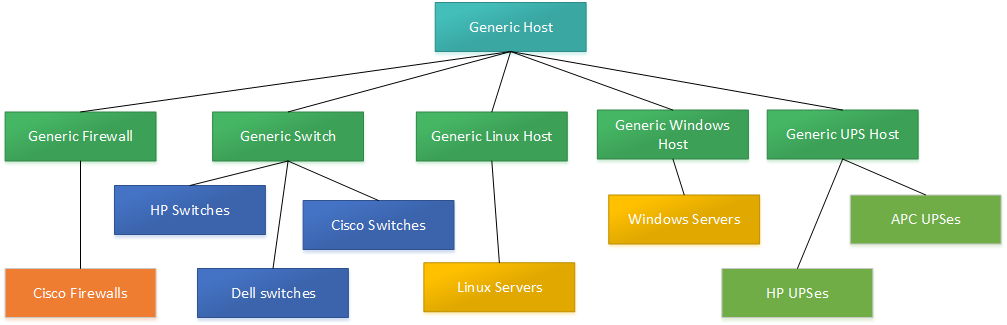
\includegraphics[scale=0.5]{img/host}
    \caption{Oversikt over host generic plassering}
    \label{hostfigur}
\end{figure}

I Figur \ref{hostgroupfigur} ser vi hvilke hostgroups de forskjellige hostene skal være medlem av.

\begin{figure}[H]
    \centering
    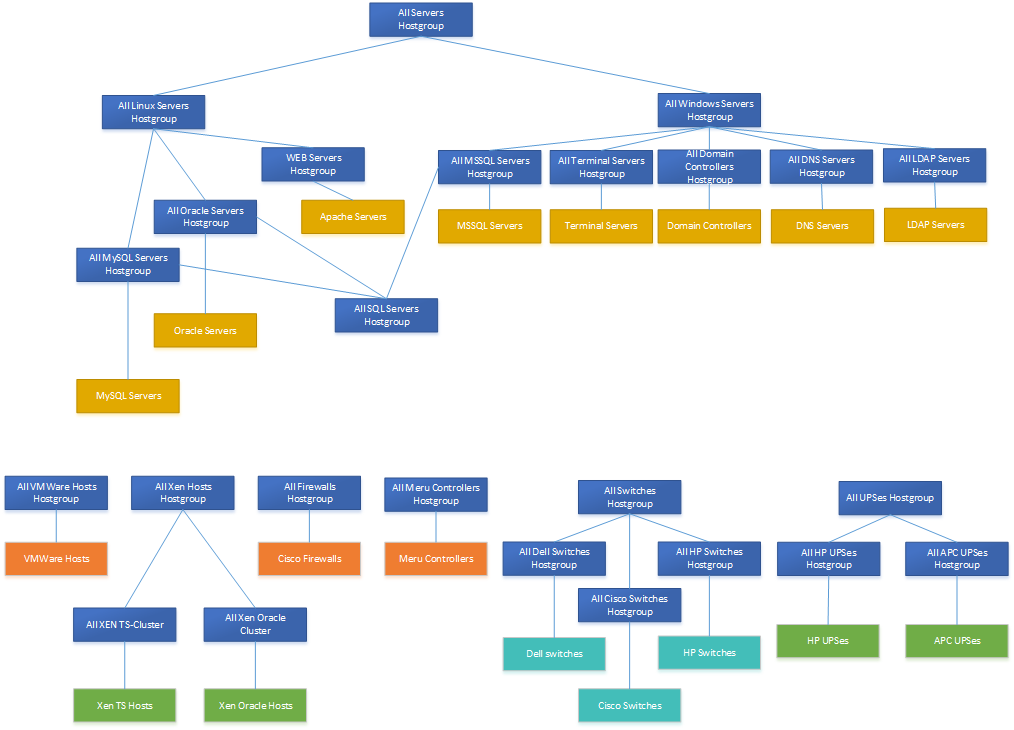
\includegraphics[scale=0.5]{img/hostgroups}
    \caption{Oversikt over hosts hostgroupplassering}
    \label{hostgroupfigur}
\end{figure}

\section{Legge til mange host-objekter}
I utrullingsfaser vil det være naturlig å legge til mange hosts på den gang. Ved å bruke "gen.bash"-scriptet spares tid samtidig som scriptet sørger for å generere hostfilene syntaktisk korrekte.

Scriptet genererer host-objekter med atributtene  ``hostname'', ``address'', ``hostgroup'' og ``generic''. Host-objekter uten hostgroup eller generic supplert, vil få standardverdier definert, mens hostname og address er obligatrisk, og det gis en feilmelding om disse er utelatt.

Eksempelet under viser hvordan scriptet kjøres og at linjenummer skrives ut dersom informasjon som er obligatorsk mangler.
\begin{lstlisting}
monkey@hig1:~/script$ vim servers.csv
monkey@hig1:~/script$ ./gen.bash servers.csv

	Generating hosts from servers.csv into working directory

	Hostname and Address are mandatory.
	Missing for host on line nr: 4
	Missing for host on line nr: 6
	Missing for host on line nr: 7
	Missing for host on line nr: 8

	Done
	Successfully created 4 hosts
	4 hosts where not created because of errors.
monkey@hig1:~/script$ ls
gen.bash  servers.csv  test1.cfg  test2.cfg  test3.cfg  test4.cfg
monkey@hig1:~/script$
\end{lstlisting}

Koden under viser hvordan servers.csv er bygget opp. Inneholder også feil for å vise hva som skjer dersom informasjonen ikke er korrekt.
\begin{lstlisting}
10.0.0.1,test1,windows;,generic1
10.0.0.1,test2,,jekrjekr
10.0.0.1,test3
,,,
10.0.0.1,test4
1,
,
,
\end{lstlisting}

Kildekoden til scriptet ligger i Vedlegg \ref{gen.bash}.

\section{Forventet nedtid}
Tilfeller kan forekomme hvor en server må tas ut av drift på grunn av vedlikehold. I Icinga er det ikke nødvendig å fjerne denne fra konfigurasjonen, for å unngå at varslingsmelding blir sendt ut. I både Icinga Web og Icinga Classic har man mulighet til å bruke en funksjon som kalles ''Schedule Downtime''. Her blir nedetidens start og slutt definert.

I den nedetidsperioden vil Icinga nekte varslingsmelding i å bli sendt ut. Når nedetidsperioden er ferdig, eller denne blir utført før avtalt tid, vil kontaktene som skal bli varslet få en melding om at nedetid er over, og Icinga vil ikke lengre holde igjen varlser.

\section{Stoppe varsling}
acknowledge, stopper gjenvarsling??
\section{Autentisering mot Active Directory} 
LDAP-autentisering brukes for å styre hvem som skal ha tilgang til web-grensesnittene, ved hjelp av grupper og brukere i Active Directory. Dette er støttet direkte i Icinga Web, men må konfigureres på andre måter for Icinga Classic. Det kan opprettes en sikkerhetsgruppe i AD som inkluderer medlemmene som skal få tilgang. Alle som er med i denne gruppen vil få tilgang til Icinga Web, der det også kan defineres hvilken informasjon hver bruker skal se. 

Selve LDAP-binden gjøres via PHP-modulen “php-ldap”. Når en bruker logger inn sjekkes først AD, dersom brukeren ikke finnes der, vil Icinga-web prøve sin egen database over brukere. Hvis brukeren finnes her og passordet er riktig vil brukeren bli logget inn. Når brukeren har logget inn for første gang via AD, vil brukeren bli lagret i Icinga Web-databasen. Om brukeren endrer passord i Icinga Web vil uansett AD først bli spurt før Icinga Web spør om passordet er riktig i sin egen database

Icinga classic autentiserer mot AD gjennom modulene ldap og authnz\_ldap.

/etc/apache2/conf.d/
\begin{lstlisting}
        AuthName "Authentication"
        AuthType Basic
        AuthBasicProvider ldap
        AuthLDAPURL
"ldap://10.60.0.22:3268/dc=monkey,dc=local?samAccountName?sub?(objectClass=person)"
        AuthLDAPBindDN "flash@monkey.local"
        AuthLDAPBindPassword "Bachel0r"
        require ldap-group CN=icinga-login, OU=icinga, DC=monkey, DC=local
\end{lstlisting}

/usr/share/icinga-web/app/modules/AppKit/config/auth.xml
\begin{lstlisting}
  <ae:parameter name="ldap_allow_anonymous">false</ae:parameter>
            <ae:parameter name="ldap_dsn">ldap://10.60.0.22</ae:parameter>
            <ae:parameter name="ldap_start_tls">false</ae:parameter>
            <ae:parameter name="ldap_basedn">DC=monkey,DC=local</ae:parameter>
            <ae:parameter name="ldap_binddn">icingawebauth@monkey.local</ae:parameter>
            <ae:parameter name="ldap_bindpw"><![CDATA[Password]]></ae:parameter>
            <ae:parameter name="ldap_userattr">sAMAccountName</ae:parameter>
            <ae:parameter name="ldap_filter_user"><![CDATA[(&(sAMAccountName=__USERNAME__)(memberOf=CN=icinga-login,OU=icinga,DC=monkey,DC=local))]]></ae:parameter>
        </ae:parameter>
\end{lstlisting}

\section{Kontakter og kontaktgrupper}

For å opprette en ny kontakt i Icinga meldes brukeren inn i gruppen icinga\_kontakter (se synkronisering). Den vil trenge å ha e-postadresse og telefonnummer satt.

Kontaktgrupper hentes fra OU-en icinga\_grupper der alle grupper hentes ut og opprettes i Icinga. For at en gruppe skal varsles må dette legges til på en service. For å slippe å sette opp kontakter for hver service kan en velge å sende med argumentet “gen\_service” for å generere en template som kan benyttes på tjenester som sorterer under hver av kontaktgruppene som blir opprettet.

Eksempel på generisk service som blir opprettet:
\begin{lstlisting}
define service {
    name network_services
    register 0
    use generic-service     
    notification_interval   30
    notification_period     24x7
    notification_options    w,c,r
    contact_groups          network_contact_group
}
\end{lstlisting}

Denne brukes på en Cisco firewall: 
\begin{lstlisting}
define service {
        service_description Cisco Firewall CPU Load
        use network_services
        name cisco-firewall-cpu-load
        hostgroup_name all_firewalls
        check_command check_network_component!cpu-load
}
\end{lstlisting}

Tabell med sjekker og tilhørende parametere:
\begin{table}
\begin{center}
\begin{tabular}{| l | l | l | l |}
 \hline
        \textbf{Utstyr} & \textbf{Service navn} & \textbf{Warning} & \textbf{Critical}
	\\ \hline
	APC UPS 		& UPS Capacity			& 90:	& 80: \\ \hline
	APC UPS			& Internal Temp			& 30	& 32 \\ \hline
	APC UPS			& Load				& 50	& 60 \\ \hline
	APC UPS			& Voltage In			& 225:239 & 220:245 \\ \hline
	APC UPS			& Voltage Out			& 225:239 & 220:245 \\ \hline 
	HP UPS			& Battery Time Remaining 	& 3000: & 2700: \\ \hline
	HP UPS			& Battery capacity		& 90: 	& 80: \\ \hline
	HP UPS			& Battery current		& 	& \\ \hline
	HP UPS			& Voltage In			& 225:239 & 220:245 \\ \hline 
	HP UPS			& Voltage Out			& 225:239 & 220:245 \\ \hline
	Windows Server		& Check DNS			& 0.1	& 0.2 \\ \hline
	Windows Server		& Check LDAP			& 0.05	& 0.1 \\ \hline 
	Windows Server		& All Disks			& 94\%	& 96\% \\ \hline
	Windows Server		& Disk Space			& 90\%	& 95\% \\ \hline
	Windows Server		& CPU Load			& 90	& 95 \\ \hline
	Windows Server		& Memory Usage			& 94\%	& 98\% \\ \hline
	Windows Server		& RDP-Sessions: Active		& 20	& 25 \\ \hline
	Windows Server		& RDP-Sessions: Inactive	& 15	& 20 \\ \hline
	Cisco ASA / PIX		& CPU Load			& 93	& 96 \\ \hline
	Cisco ASA / PIX		& Hardware Health		& N/A	& N/A \\ \hline
	Cisco ASA / PIX		& Memory Usage			& 93	& 96 \\ \hline
	Cisco ASA / PIX		& Failover Status		& N/A	& N/A \\ \hline
	Cisco ASA / PIX		& VPN Sessions			& 80 (\% av lisens) & 90 (\% av lisens) \\ \hline
	Dell Blade Chassis	& Dell Blade Server Health	& N/A	& N/A \\ \hline
	Dell Powerconnect	& Assets			& N/A	& N/A \\ \hline
	Dell Powerconnect	& Uptime			& N/A	& N/A \\ \hline
	Dell Powerconnect	& Fans				& N/A	& N/A \\ \hline
	Dell Powerconnect	& Power supply			& N/A	& N/A \\ \hline
	Dell Powerconnect	& Temperature			& 34	& 36 \\ \hline
	HP Procurve		& Environment Status		& N/A	& N/A \\ \hline
	MySQL			& Cache Hit			& 60: 	& 50: \\ \hline
	MySQL			& Health			& 0.1	& 0.2 \\ \hline
	MySQL			& Slow Queries			& 0.1	& 1 \\ \hline 
	MySQL			& User Connections		& 50	& 80 \\ \hline
	MSSQL			& Cache Hit			& 90:	& 80: \\ \hline
	MSSQL			& Health			& 0.05	& 0.15 \\ \hline
	MSSQL			& Lazy Writes			& 20	& 0 \\ \hline
	MSSQL			& User Connections		& 2000	& 2200 \\ \hline
	Oracle			& Cache Hit			& 93:	& 90: \\ \hline
	Oracle			& Connected Users		& 50	& 80 \\ \hline
	Oracle			& Connection Time		& 0.1	& 0.2 \\ \hline
	Oracle			& Free Tablespace		& 5:	& 2: \\ \hline
\end{tabular}
\label{objekt_varsling}
\end{center}
\end{table}
